\documentclass[tikz,14pt,fleqn]{article}

% Math
\usepackage[fleqn]{amsmath}
\usepackage{amssymb}
\usepackage{gensymb}
\usepackage{dsfont}
\usepackage{float}

% Insert dummy text
\usepackage{lipsum}  
% Allows to use caption*
\usepackage{caption}
% Scalable subfigures and subcaptions
\usepackage{subcaption} 
% Wrap text around figures
\usepackage{wrapfig}
% Code syntax highlighting
\usepackage{minted}
% Hyperlinks
\usepackage{hyperref}
% Customize page layout
\usepackage{geometry}
\geometry{a4paper, margin=1in}
% Page headers and footers
\usepackage{fancyhdr}
\pagestyle{fancy}
\fancyhf{}
\setlength{\parindent}{0pt}
\setlength{\parskip}{0.5\baselineskip}%

% includegraphics
\usepackage{graphicx}


\usepackage{cleveref}

\newcommand{\bmat}[1]{
   \ensuremath{
   \begin{bmatrix}
       #1
   \end{bmatrix}
}}
\newcommand{\pmat}[1]{
   \ensuremath{
   \begin{pmatrix}
       #1
   \end{pmatrix}
}}

\usepackage{hyperref}



\usepackage[utf8]{inputenc}


%%%%%%%%%%%%%%%%%%%%%%%%%%%%
%% VARIABLES
\newcommand\namesurname{Albert Cerfeda}
\newcommand\assignment{Assignment 1 - Linear Regression}

\newcommand\subject{Machine Learning}
\newcommand\documentdate{27 April 2023}

% Title content
%%%%%%%%%%%%%%%%%%%%%%%%%%%%
\rhead{\assignment}
\lhead{\namesurname}
%%%%%%%%%%%%%%%%%%%%%%%%%%%%

\rfoot{Page \thepage}


\begin{document}

\begin{titlepage}
   \begin{center}
       \vspace*{0.2cm}

       \textbf{\Large{\subject}}

       \vspace{0.5cm}
        \textbf{\assignment}\\[5mm]
        
            
       \vspace{0.4cm}

        \namesurname
        \begin{figure}[H]
            \centering
        \end{figure}
       \tableofcontents

       \vspace*{\fill}
     
        
\includegraphics[width=0.4\textwidth]{fig/logo.png}
       
        \documentdate \\
        Università della Svizzera italiana\\
        Faculty of Informatics\\
        Switzerland\\

   \end{center}
\end{titlepage}


\section{Tasks}

This section should contain a detailed description of how you solved the assignment, including all required statistical analyses of the models' performance and a comparison between the linear regression and the model of your choice. Limit the assignment to 8-10 pages and do not include any code in the report.

\subsection{Task 1}
Use the family of models $f(\mathbf{x}, \boldsymbol{\theta}) = \theta_0 + \theta_1 \cdot x_1 + \theta_2 \cdot x_2 + \theta_3 \cdot \sin(x_2) + \theta_4 \cdot x_1 \cdot x_2$ to fit the data. 
\begin{wrapfigure}{l}{0.20\linewidth}
    \centering
    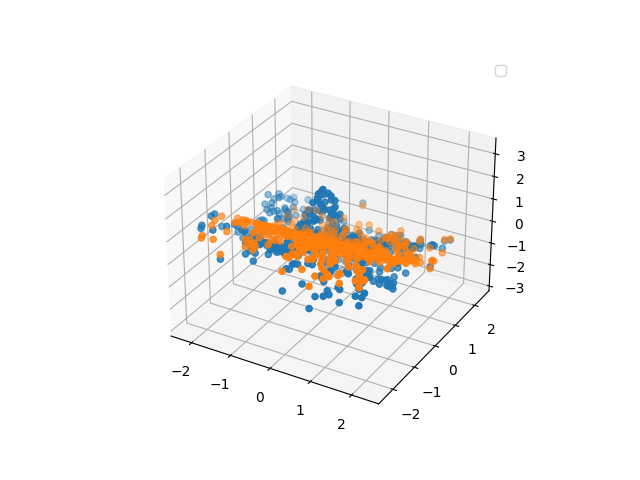
\includegraphics[width=1\linewidth]{fig/out/T1.predictions.png}
    \vspace{-1.35cm}
    \label{fig:1.1}
\end{wrapfigure}
% TODO: Explain model
\begin{itemize}
	\item [a.] Write in the report the formula of the model substituting parameters $\theta_0, \ldots, \theta_4$ with the estimates you've found:
	$$f(\mathbf{x}, \boldsymbol{\theta}) = (0.00205) + (0.04164) \cdot x_1 + (0.13866) \cdot x_2 + (-1.21627) \cdot \sin(x_2) + (0.05262) \cdot x_1 \cdot x_2$$
	\item [b.] Evaluate the test performance of your model using the mean squared error as performance measure.\\
	Mean Squared Error (MSE) on the Test set: 0.48117
\end{itemize}
\subsection{Task 2}
Consider any family of non-linear models of your choice to address the above regression problem.
\begin{wrapfigure}{l}{0.20\linewidth}
    \centering
    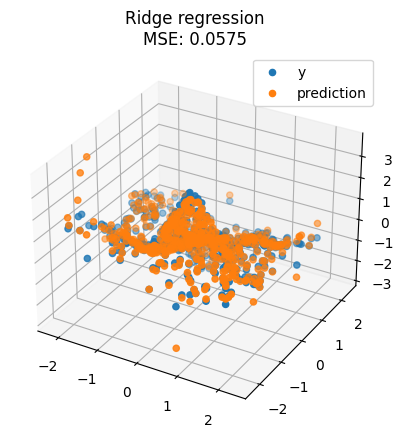
\includegraphics[width=1\linewidth]{fig/out/T2.predictions.png}
    \vspace{-1.7cm}
    \label{fig:1.1}
\end{wrapfigure}
%  TODO: Explain model
\begin{itemize}
	\item [a.] Evaluate the test performance of your model using the mean squared error as performance measure.\\
    Mean Squared Error (MSE) on the Test set: 0.05747
	\item [b.] Compare your model with the linear regression of Task 1. Which one is {statistically} better? \\
	Comparing the MSE of the two models, we can see that the non-linear model performs better than the linear one. % TODO: Why does it perform better ?
\end{itemize}

\subsection{Task 3 (Bonus)}

In the \href{https://github.com/GiorgiaAuroraAdorni/ML-bachelor-course-assignments-sp23}{\textbf{GitHub repository of the course}}, you will find a trained Scikit-learn model that we built using the same dataset you are given. 
This \textit{baseline} model is able to achieve a MSE of \textbf{0.022}, when evaluated on the test set. 
You will get extra points if you provide a model of your choice whose test performance is \textbf{better} (i.e., the MSE is lower) than ours. Of course, you must also tell us why your model is performing better.
\begin{wrapfigure}{l}{0.20\linewidth}
    \centering
    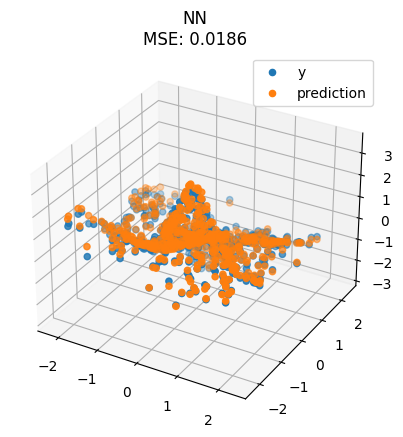
\includegraphics[width=1\linewidth]{fig/out/T3.predictions.png}
    \vspace{-1.5cm}
    \label{fig:1.1}
\end{wrapfigure}
As mentioned in the exercise text, the baseline model achieves a MSE of \textbf{0.022} on the test set. \\ The simple neural network I used, once trained on the training set and evaluated on the test set achieves a MSE of \textbf{0.01863}, lower than the baseline model. The neural network has 4 subsequent dense layers with 64 nodes each. The activation functions of each layer (in order) are: Exponential Linear Unit, Rectified Linear Unit, Sigmoid and Linear. \\
%----------------------------------------------------------------------------------------
%	Questions
%----------------------------------------------------------------------------------------
%\newpage
\section{Questions}

\subsection{Q1. Training versus Validation}
\begin{figure}[h!]
    \centering
    \vspace*{-0.5cm}
    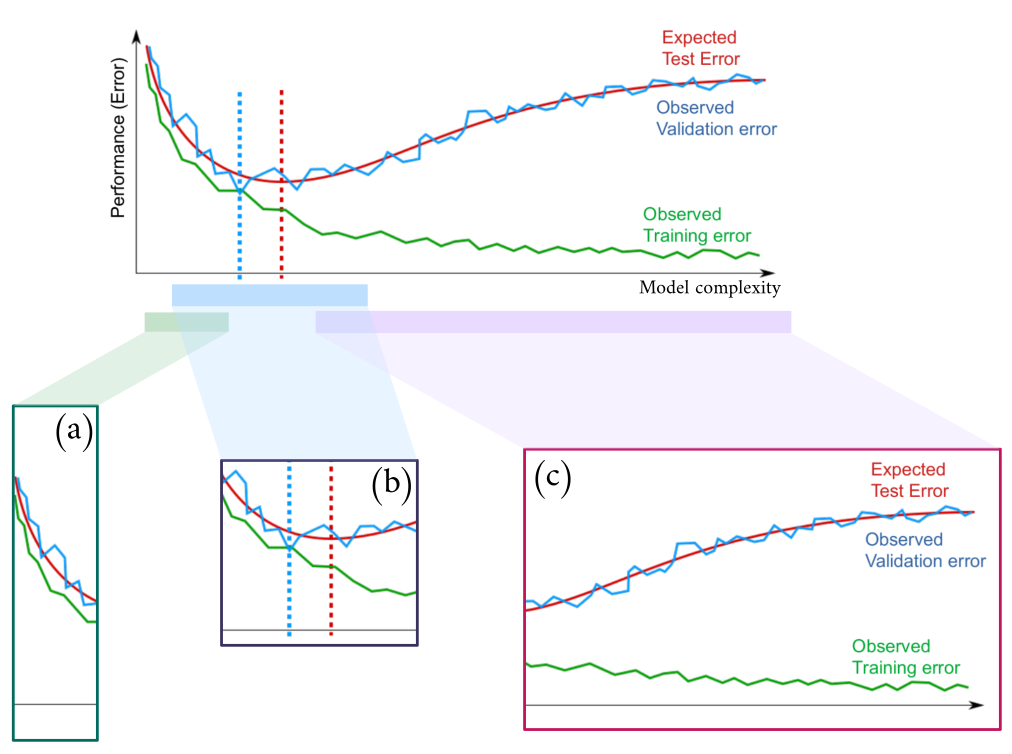
\includegraphics[width=0.5\linewidth]{fig/ex_train_val_test.png}
    \vspace*{-0.3cm}
    \caption{Error estimates related to model complexity}
    \vspace*{-0.3cm}
    \label{fig:q1}
\end{figure}
\begin{itemize}
\item[Q1.1] \textbf{What is the whole figure about?}
\item[A1.1] The figure shows how the Test Error, Training Error and Validation Error change based on the model complexity. The graph demonstrates how the error estimates are not actually monotonically increasing/decreasing but overall tend to grow or shrink as the complexity increases.\\
We can see as how the training error tends to decrease with more complex models. That is because the model, having more parameters, has greater flexibility to learn the complex patterns of data. As our predictions get closer and more accurate, our test error increases as the model has learned the training data "too well" and therefore is not able to predict new, previously unseen data (overfitting).
\item[Q1.2] \textbf{Explain the behaviours of the curves in each of the three highlighted sections in the figure, namely (a), (b), and (c).}   
\item[A1.2] The three subfigures highlight three separate phases related to the model complexity or the training phase. Subfigure \verb|a)| shows the case in which the model is too simple, where the error estimates are high and quickly decreasing as the model complexity increases. Choosing the model complexity in this phase would be premature as the model is not capable to approximate the function generating the data (i.e underfitting). Subfigure \verb|b)| shows the situation where the model has an optimal complexity. We can see that the test error has reached a minimum, after which it will start increasing again. This means that the model is not running into loss of generalizability yet and did not incur in overfitting. Finally, in the last picture we can clearly see how the model is complex enough to approximate the noise of the data and is incurring into overfitting. That is, the model is really good at predicting the biased training data and is not able to predict never-seen-before data.
\begin{itemize}
\item[Q1.2.a] \textbf{Can you identify any signs of overfitting or underfitting in the plot? If yes, explain which sections correspond to which concept.}
\item[A1.2.a] As previously stated, we can see underfitting happening in Subfigure \verb|a)| and overfitting happening in picture \verb|c)|.
\item[Q1.2.b] \textbf{How can you determine the optimal complexity of the model based on the given plot ?}
\item[A1.2.b] The validation set is used for model selection. When performing model selection, we choose the one that minimizes the validation error. We may not use the test set instead of the validation set for model selection, as minimizing the test error would lead in overfitting it and therefore in a biased performance measure after the model has been trained.
The red dashed line in Subfigure \verb|b)| represents the actual optimal model. By using the validation set for model selection we notice how we are able to estimate the optimal model complexity.
\end{itemize}
\item[Q1.3] \textbf{Is there any evidence of high approximation risk? Why? If yes, in which of the below subfigures?} 
\item[A1.3] The approximation risk is the error between the true funtion that generates the data and our model that tries to approximate it. In other words, the approximation risk is the error that results from choosing a model that is not complex enough to capture the true underlying relationship between the inputs and the outputs. This can result in the model being too simple and underfitting the data. We can therefore infer how Subfigure \verb|a)| has a high approximation error.
\item[Q1.4] \textbf{Do you think that increasing the model complexity can bring the training error to zero? And the structural risk ?}
\item[A1.4] It is possible to make the training error converge to 0 by increasing the model complexity, however it would not be a good idea in a real world scenario as the goal of the learning procedure is to imitate the real function generating the data. The structural risk, also known as the bias error, is the error that results from the limitations of the model class and its inability to represent the true underlying function. This error can only be reduced by selecting an appropriate model architecture that can capture the complexity of the underlying function, rather than by simply increasing the complexity of the model.
\item[Q1.5] \textbf{If the X axis represented the training iterations instead, would you think that the training procedure that generated the figure used early stopping? Explain why.} (\textbf{NB:} ignore the subfigures and the dashed vertical lines)
\item[A1.5]  No. The idea is to monitor the performance of the model on a validation set (a separate portion of the data that is not used for training), and stop the training process when the performance on the validation set starts to deteriorate. This stops the training early before the model starts overfitting the data. Clearly early stopping has not been employed as the model has been trained well into overfitting.
\end{itemize}

\subsection{Q2. Linear Regression}
Comment and compare how the (a.) training error, (b.) test error and (c.) coefficients would change in the following cases:
\begin{itemize}
\item[Q2.1] \textbf{$x_3 = x_1 + 0.2 \cdot x_2$.}
\item[A2.1] In this case, the new feature $x_3$ is represented as a linear combination of the two
already-existing features $x_1$ and $x_2$ and is dependent on them. Adding this new
feature to the family model, it changes to $f(x,\theta) = \theta_0 + \theta_1 x_1 + \theta_2 x_2 + \theta_3(x_1 + 0.2x_2)$. When we add a new feature $x_3$ to the model, which is a linear combination of the existing features $x_1$ and $x_2$, the training error may decrease as the model has more information to learn from. However, adding $x_3$ can lead to \textit{multicollinearity}, which occurs when two or more predictor variables are highly correlated with each other. In this case, since $x_3$ is dependent on both $x_1$ and $x_2$, the new feature can introduce multicollinearity, which can make it difficult to determine the individual effect of each feature. This can cause the coefficients of $x_1$ and $x_2$ to become unstable and difficult to interpret, with $x_3$ dominating and having a larger impact on the predicted values of the target variable.
Multicollinearity can also lead to over-fitting, where the model may perform well on the training set but fail to generalize to new, unseen data. This can cause the test error to increase and decrease the model's overall performance. Additionally, multicollinearity can cause unpredictable variance and decrease the statistical significance value, making it difficult to determine how important a feature is to the target variable.
To mitigate the problem of multicollinearity, Ridge regression can be used. Ridge regression adds a penalty term to the cost function, which shrinks the magnitude of the coefficients of the predictor variables, forcing them to be smaller. This helps to stabilize the coefficients and improve the model's performance on new, unseen data.

\item[Q2.2] \textbf{$x_3 = x_1 \cdot x_2 \cdot x_2$}
\item[A2.2] When we add a new feature $x_3$ which is a non-linear combination of features $x_1$ and $x_2$, the model changes to a quadratic polynomial of the form $f(x, \theta) = \theta_0 + \theta_1 x_1 + \theta_2 x_2 + \theta_3 x_1 x_2$. The coefficients $\theta$ are still positively related, so $x_3$ is expected to be positively correlated with the target variable $y$.
Adding a new feature $x_3$ can introduce new interactions between $x_1$ and $x_2$ that were not apparent in the linear representation. This non-linear relationship between $x$ and $y$ can potentially improve the model's approximation of the true function $g(x)$, which can lead to better performance and a reduction in testing error.
If the correlation between $x_1$ and $x_2$ is significant, adding the new feature can improve performance, but if the correlation is not significant, adding the new feature may not result in any significant improvement. Ultimately, the impact of adding the new feature on the training error, testing error, and coefficients depends on the specifics of the dataset and the relationship between the variables.

\item[Q2.3] \textbf{$x_3$ is a random variable independent from $y$.}
\item[A2.3] By adding feature $x_3$ , that is independent of the target variable $y$, the model will have new parameter $\theta_3$, that is not useful for predicting $y$. This is because $x_3$ holds no significant information or predictive power for the target variable. As a result, adding such features to the model does not improve its performance and only increases its complexity, which can lead to overfitting. The training error may decrease with the addition of the new feature, but the testing error will likely increase, as the model will be overfit to the training data.

\item[Q2.3] \textbf{How would your answers change if you were using Lasso Regression?}
\item[A2.3] Lasso is a regression variant which features a slightly different loss function:
$$
V_{\text {Lasso }}(\theta)=\frac{1}{n} \sum_{i=1}^n\left(y_i-x_i^T \theta\right)^2+\lambda \sum_{i=2}^d\left|\theta_i\right|
$$
Notice how a penalty term for large parameters has been introduced, shrinking some of the parameters to zero and performing feature selection.
If the new variable, $x_3$, is a linear combination of $x_1$ and $x_2$, adding it to the model may cause the coefficients of $x_1$ and $x_2$ to be reduced to zero, especially if the regularization parameter $\lambda$ is high. This is because multicollinearity is introduced, and Lasso penalizes coefficients with highly correlated features. Thus, adding $x_3$ may not improve model performance.

On the other hand, if $x_3$ is a non-linear combination of $x_1$ and $x_2$, adding it may lead to non-zero coefficients for all three features, since Lasso can handle non-linear relationships between features and the target variable. However, the magnitude of the coefficient of $x_3$ may be smaller than that of the original features, especially if the non-linearity of the relationship between $x_3$ and the target variable is not strong enough to justify its inclusion in the model.

\item[Q2.4] \textbf{Explain the motivation behind Ridge and Lasso regression and their principal differences.}
\item[A2.4] Ridge and Lasso regression are two commonly used techniques in regression analysis that can help prevent overfitting and reduce model complexity. When we use simple linear regression, we risk overfitting the model to our data, which can lead to poor performance on new data.
$$
V_{\text {Ridge }}(\theta)=\frac{1}{n} \sum_{i=1}^n\left(y_i-x_i^T \theta\right)^2+\lambda\|\theta\|^2
$$
Ridge regression modifies the cost function by adding a penalty term that is equal to the squared norm of the coefficient vector. This penalty term, also known as the regularization parameter, results in the coefficients being generally smaller, reducing model complexity and multicollinearity.

Lasso regression as we have seen before also adds a penalty term for the coefficients. However by penalizing the sum of their absolute values, it favours individual parameters going exactly to 0.

In addition to reducing overfitting and model complexity, Lasso regression can also be used for feature selection. However, the optimization problem for lasso regression is not convex, meaning that quadratic programming methods are needed to solve the minimization problem.
\end{itemize}

\subsection{Q3. Classification}
\begin{figure}[h!]
    \centering
    \vspace*{-0.5cm}
    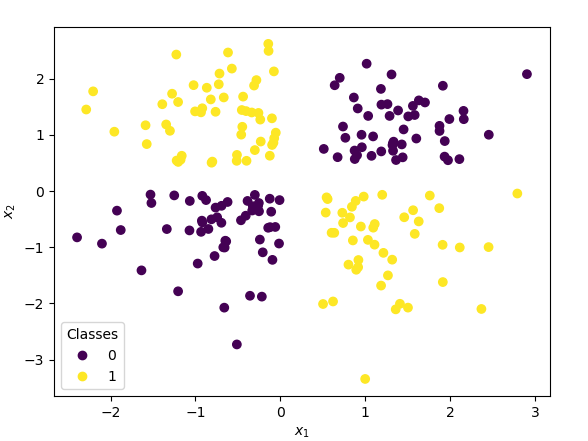
\includegraphics[width=0.7\linewidth]{fig/clustering.png}
    \vspace*{-0.3cm}
    \caption{Dataset and its data classes}
    \vspace*{-0.3cm}
    \label{fig:q3}
\end{figure}
\begin{itemize}
\item[Q3.1] \textbf{Your boss asked you to solve the problem using a perceptron, and now he's upset because you are getting poor results. How would you justify the poor performance of your perceptron classifier to your boss?}
\item[A3.1] The working principle of the perceptron algorithm is classyfing data points into two classes based on a \textit{linear} decision boundary. That is, the data is clustered based on a hyperlane that separates the two classes. During training the perceptron applies the activation function with its weights and features and clusters the data. In the case of the dataset in Figure \ref{fig:q3}, the data is not linearly separable, and thus the perceptron algorithm will not be able to classify the data points correctly. That is, the pattern of the data grouped together into 4 separate clusters is too complex for the perceptron to correctly detect and classify.

\item[Q3.2] \textbf{Would you expect better luck with a neural network with the activation function $h(x) = - x * e^{-2}$ for the hidden units?}
\item[A3.2] The activation function $h(x) = - x * e^{-2}$ is a sigmoid function, which is a non-linear function. Using a linear activation funcion for a Neural Network makes it behave like a regular Linear Regression. As such, it is not fit for solving non-linear problems. We can therefore not expect the performance to get better.

\item[Q3.3] \textbf{What are the main differences and similarities between the perceptron and the logistic regression neuron?}
\item[A3.3] Both of them are usually employed for solving binary clustering problems. The perceptron gives only a binary classification (e.g \verb|Set 1| / \verb|Set 2|). The Logistic regression neuron is more advanced as it also provides the probability for each data class (e.g \verb|Set 1| - $70\%$).

\end{itemize}


\end{document}